%%%%%%%%%%%%%%%%%%%%%%%%%%%%%%%%%%%%%%%%%%%
%%%%%%  STYLE 12
%%%%%%%%%%%%%%%%%%%%%%%%%%%%%%%%%%%%%%%%%%%
\cxset{style12/.style={
 name={},
 numbering=arabic,
 number font-size=\HUGE,
 number font-family=\rmfamily,
 number font-weight=\bfseries,
 number before=,
 number dot=,
 number color=\color{gray},
 number after=\par,
 number position=rightname,
 chapter font-family=\sffamily,
 chapter font-weight=\normalfont,
 chapter font-size=\Huge,
 chapter before={\raggedright\par},
 chapter after={},
 chapter color={black!90},
 title beforeskip={\vspace*{30pt}},
 title afterskip={\vspace*{50pt}\par},
 title before={},
 title after={\par\vspace{30pt}\rule{\textwidth}{4pt}},
 title font-family=\sffamily,
 title font-color=\color{purple},
 title font-weight=\bfseries,
 title font-size=\HUGE,
 title spaceout=none,
}}


\cxset{style12}
\chapter{Introduction to \\ Style Twelve}

This is a variation of Style 7, with only the lettering and the rule are thicker. In my opinion it looks better with a bit of color, so I have used a purple color with a gray.

\medskip
\begin{figure}[ht]
\centering
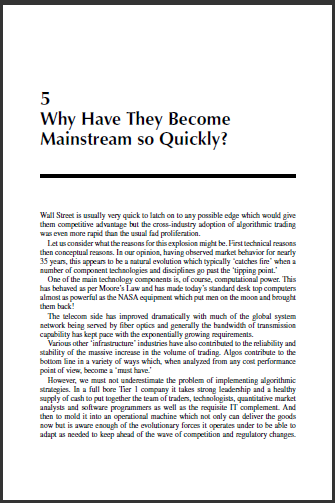
\includegraphics[width=0.35\textwidth]{./chapters/chapter12}
\end{figure}
\lipsum[1]
